\section{Desarrollo}

\subsection{Elección de Destinos}

Para realizar los experimentos se eligieron 3 universidades de distintos continentes para así poder presentar variedad en las rutas examinadas y poder analizar, luego, cuánto impactan los enlaces transatlánticos. En el Cuadro~\ref{tab:infouniv} se muestra la información de dichos destinos. Para el cálculo teórico del \textit{RTT}, las distancias se estimaron entre ciudad origen de los experimentos (\textsl{Ciudad Autónoma de Buenos Aires, Argentina}) y las respectivas ciudades de las universidades destino. Para ello se utilizó la herramienta de cálculo implementada en \textit{GeoBytes} \footnote{http://www.geobytes.com/citydistancetool.htm}. En la figura~\ref{fig:mapuniv1} se graficaron en un mapa los respectivos puntos con una estimación gráfica de la distancia lineal entre ellos.\\

\begin{table}[h]
    \centering
    \begin{tabular}{ | c | c | c | c | c |}
	    \hline
	    \textbf{Universidad} & \textbf{URL} & \textbf{IP} & \textbf{Continente} & \textbf{Distancia \textit{(km)}}\\ \hline
	    Univ. de California, Berkeley & http://www.berkeley.edu & 169.229.216.200 & América & 10412\\ \hline
	    Univ. de Oxford & http://www.ox.ac.uk & 163.1.60.42 & Europa & 11107\\ \hline
	    Universidad de Tokio & http://www.u-tokyo.ac.jp & 59.106.161.11 & Asia & 18372\\ \hline
    \end{tabular}
    \caption{Información sobre Universidades destino elegidas.}
    \label{tab:infouniv}
\end{table}

\begin{figure}[h!]
  \centering
  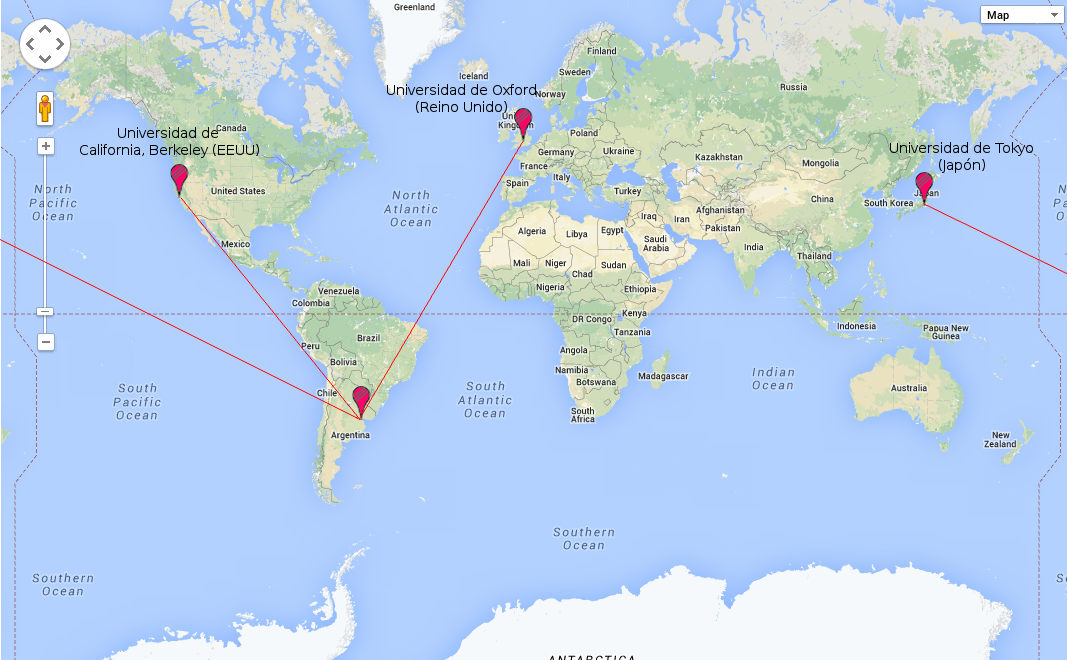
\includegraphics[width=0.7\textwidth]{./figs/map-univs1.png}
  \caption{Localización del origen y destinos con las respectivas distancias lineales aproximadas}
  \label{fig:mapuniv1}
\end{figure}

\subsection{Implementación de \textsl{Traceroute}}

El objetivo de la herramienta \textsl{traceroute} es examinar y trazar una porción de la ruta que atraviesa un paquete desde un origen hasta cierto destino a lo largo de las distintas redes por las que navega. Si bien tanto el sistema operativo Linux como la biblioteca de \textit{Python}, \textsl{Scapy}, proveen robustas implementaciones de esta utilidad, en principio no aplican para tomar tiempos, entre ellos el \textit{RTT}. Es por eso que se procedió a una implementación propia de \textsl{traceroute} basado en el enfoque de envío de paquetes \textit{ICMP}. En un \textit{ping} tradicional, dado un origen y un destino, el primero envía un paquete IP junto con un mensaje ICMP de tipo \textit{echo-request} a la espera de una respuesta satisfactoria de tipo \textit{echo-reply}. Para que esto suceda con éxito, el paquete ip debe tener un valor suficientemente grande en su campo \textit{ttl - time to live} de modo que los distintos nodos de la ruta lo reenvien hacia destino. En caso de que ese campo no sea suficiente para que el paquete llegue al destino deseado, el nodo que detecta el agotamiento de su \textit{ttl} responde con un mensaje ICMP de tipo {time-exceeded}. Tomando esta característica de la transmisión de paquetes y mensajes ICMP, la idea detrás de esta implementación de traceroute consiste en realizar sucesivos envíos de un paquete IP + mensaje ICMP \textit{echo-request} a destino comenzando con un \textit{ttl} unitario e incrementándolo en uno. De esta manera, el paquete 'muere' en distintos puntos del tramo y se puede identificar algunos de los nodos que se atraviesan ya que estos proveen su información al responder \textit{time-exceeded}.\\
